\documentclass{article}

\usepackage{amsmath}
\usepackage[margin=0.1in]{geometry}
\usepackage{booktabs}
\usepackage{tipa}
\usepackage{amssymb}
\usepackage{dsfont}
\usepackage{tikz}
\usetikzlibrary{fit}
%\usepackage{color}
\usepackage[dvipsnames]{xcolor}
\usepackage{multirow}
\usepackage{hyperref}
\usepackage{amsfonts}       % blackboard math symbols
\usepackage{phonrule} 
 % For algorithms
\usepackage{algorithm}
\usepackage{algorithmic}

\title{Automatically Exploring Hypothesis Spaces}
%\author{Kevin Ellis, Timothy O'Donnell}

\newcommand{\nextForm}[1]{\rotatebox[origin=c]{270}{$_{\curvearrowright}$}$_{#1}$}
\DeclareMathOperator*{\argmin}{arg\,min}
\newcommand{\Expect}{\mathds{E}} %{{\rm I\kern-.3em E}}
\newcommand{\indicator}{\mathds{1}} %{{\rm I\kern-.3em E}}
\newcommand{\expect}{\mathds{E}} %{{\rm I\kern-.3em E}}
\newcommand{\probability}{\mathds{P}} %{{\rm I\kern-.3em P}}

\begin{document}
\maketitle


\section{Automatically generating grammars with Bayesian program learning}

\subsection{A Probabilistic Framing}

A goal of the grammar learner, whether it is a child, linguist, or computer program, is to
infer the grammar that gave rise to
a collection of utterances.
One way of
modeling this inference problem is to (1) place a prior distribution over grammars, for example, a distribution that puts more probability mass on shorter or simpler grammars; (2) equip each grammar with a
\emph{likelihood model} that specifies exactly how likely a grammar is to produce a given utterance;
and then (3) use Bayes's rule to work backwards from the
utterances to the grammar that was likely to produce them:
\begin{equation}
  \probability\left[\text{grammar}|\text{utterances} \right]\propto\underbrace{\probability\left[\text{utterances}|\text{grammar} \right]}_{\text{Likelihood}}\times\underbrace{\probability\left[\text{grammar} \right]}_{\text{Prior}}\label{posterior}
\end{equation}
We can think of the above equation as a recipe for
scoring how well a grammar explains a
collection of utterances.
Once we have a prior and a likelihood,
we know how to evaluate how well a grammar explains the data, modulo the assumptions implicit in the
prior and likelihood.
In this work we will use this probabilistic framing
to explore spaces of grammars
that an AGL learner could use to explain
the pronunciations of words.
Here the grammars will be SPE-style rewrite rules~\cite{chomsky1968sound},
commonly used in generative phonology,
but at a high level this framing can apply to
learning other aspects of grammar like semantics~\cite{piantadosi2011learning}, syntax~\cite{perfors2011learnability}, and morphology~\cite{tim}.

\noindent\textbf{SPE-style rewrite notation:} Each SPE-style rewrite rule is a function that both inputs and outputs a sequence of phonemes.
These rewrites are written as ``\phonb{input}{output}{left}{right}'' %$\text{input}\to\text{output }/\text{ left } \_ \text{ right}$'',
which means that ``input'' gets rewritten to ``output'' whenever ``left'' is to the left and ``right'' is to the right.
Some special symbols used in these rules are \# to mean the start or end of the input;
C/V to mean a consonant/vowel; $\sigma $ to mean a syllable;
and $\varnothing$ to mean the empty string.
For example, the rule
\phonb{$\sigma $}{$\varnothing$}{\#}{C}
deletes a syllable at the start of a word if it is followed by a consonant.
Rules can refer to sets of phonemes by writing down vectors of phonological features -- for example,
the rule \phon{[-son]}{[+voice]} rewrites segments that are -sonorant (e.g., \textipa{k,d,v,S,...}) to their voiced counterparts (e.g., \textipa{g,d,v,Z,...}).
Rules can also bind variables to phonemes or syllables,
which are written using subscripts;
for example,
\phonr{C$_i$}{$\varnothing$}{C$_i$}
%$\text{\texttt{C}}_i\to\varnothing / \_ \text{\texttt{C}}_i$
deletes a consonant if it is followed by the same consonant,
and
\phonb{$ \varnothing $}{$\sigma _i$}{#}{$\sigma _i$}
%$\varnothing\to\sigma_i / \text{\texttt{\#}}\_\sigma_i$
inserts a copy of a word initial syllable.
The special subscript ``0" means zero or more occurrences of the subscripted segment,
so for example \phonl{V}{[+hi]}{[+hi][ ]$_0$} means that vowels become +hi whenever there exists a +hi phoneme anywhere to the left.

\noindent \textbf{Prior \& Likelihood:} A simple and intuitive prior over grammars is one which penalizes longer grammars and favors parsimonious grammars, for example defining $\probability\left[\text{grammar} \right]\propto\exp\left(- \text{\# symbols in grammar} \right)$. An example of a likelihood model,
and the one we use here,
is just to count the number of extra bits or symbols needed to encode an utterance given the grammar\footnote{This is equivalent to a minimum description length (MDL) interpretation}.

Now in theory this probabilistic framing
has now bought us a procedure for automatically discovering
grammars that do a good job explaining the data.
In practice,
the space of all grammars is infinite and combinatorial,
and so cashing out this framing requires a
efficient procedure for searching the space of grammars and honing in on those that maximize Equation~\ref{posterior}.
A subfield of computer science, called \textbf{program synthesis},
has developed efficient techniques for
solving seemingly intractable combinatorial search problems
like those that arise in grammar learning.
We use a program synthesis tool called Sketch~\cite{solar2008program}
to search for grammars maximizing~\ref{posterior},
which was previously applied to language learning problems in~\cite{ellis2015unsupervised}.
For more detail on these program synthesis techniques we refer the reader to~\cite{solar2008program}.
This cashing out of the framing makes
our approach an instance of  \textbf{Bayesian Program Learning (BPL)}; see~\cite{lake2015human}.


\subsection{Modeling solutions to AGL problems}


The fundamental hypothesis underlying AGL research is that
artificial grammar learning must engage some shared resource with first language acquisition --
and so we can gain insights into first language acquisition by
instead studying AGL in controlled experiments.
Our demonstration here is that
a BPL model can explain how a learner can quickly (e.g., from very little data) infer a grammar represented as SPE--style rules.
We collected grammars from AGL datasets~\cite{gerken2010infants,marcus1999rule,frank2011three}
and presented our BPL learner with data drawn from these grammars (Table~\ref{artificialGrammarTable}),
finding that our model automatically discovers the grammars that
 underly these data sets.
\begin{table}[h!]
\centering\begin{tabular}{lcll}
  \toprule
  Grammar&\begin{tabular}{c}
    Example input \\to learner
    \end{tabular}&Inferred grammar&Natural language analogues\\\midrule
  \begin{tabular}{l}
    ABA \\
  Marcus et al. 1999.     
    \end{tabular}&
  \begin{tabular}{l}
    wofewo\\
    lovilo\\
    fimufi
  \end{tabular}&
  \begin{tabular}{l}
    \phonb{$\varnothing $}{$\sigma _i$}{\#}{$\sigma \sigma _i$}
%$\varnothing\to \sigma_i/$\texttt{\#\_}$\sigma \sigma_i$
  \end{tabular}& Reduplication (eg, Tagalog)
  \\\midrule
  \begin{tabular}{l}
      ABB\\
  Marcus et al. 1999. 
    \end{tabular}&
  \begin{tabular}{l}
        wofefe\\
    lovivi\\
    fimumu
  \end{tabular}&
  \begin{tabular}{l}
    \phonb{$\varnothing $}{$\sigma _i$}{$\sigma _i$}{\#}
    %$\varnothing\to \sigma_i/\sigma_i$\texttt{\_\#}
  \end{tabular}&
  Reduplication (eg, Tagalog)\\\midrule
  \begin{tabular}{l}
      ABx 
    \end{tabular}&
  \begin{tabular}{l}
        wofeka\\
    lovika\\
    fimuka
  \end{tabular}&
  \begin{tabular}{l}
stem$+x$
  \end{tabular}&concatenative morphology
  \\\midrule
  \begin{tabular}{l}
    AAx \\Gerken 2006. %~\cite{gerken2010infants}
    \end{tabular}&
  \begin{tabular}{l}
        wowoka\\
    loloka\\
    fifika
  \end{tabular}&
  \begin{tabular}{l}
    stem+$x$\\
    \phonb{$\varnothing $}{$\sigma _i$}{\#}{$\sigma _i$}
%$\varnothing\to \sigma_i/$\texttt{\#\_}$\sigma_i$
  \end{tabular}&
  \begin{tabular}{l}
    reduplication\\concatenative morphology
    \end{tabular}\\\midrule
  \begin{tabular}{l}
    AxA \\Gerken 2006. %~\cite{gerken2010infants}
    \end{tabular}&
  \begin{tabular}{l}
        wokawo\\
    lokalo\\
    fikafi
  \end{tabular}&
  \begin{tabular}{l}
    $x+$stem\\
    \phonb{$\varnothing $}{$\sigma _i$}{\#}{$\sigma \sigma _i$}
    %$\varnothing$ $\to\sigma_i/$\texttt{\#\_}  $\sigma$ $\sigma_i$
  \end{tabular}&
  \begin{tabular}{l}
    Infixing\\Reduplication
    \end{tabular}
  \\\midrule
  \begin{tabular}{l}
    Pig Latin
    \end{tabular}&
  \begin{tabular}{l}
    \textipa{pIg}$\to$\textipa{Igpe}\\
    \textipa{latIn}$\to$\textipa{atIle}\\
    \textipa{\ae sk}$\to$\textipa{\ae ske}\\
  \end{tabular}&
  \begin{tabular}{l}
    \phonb{$\varnothing $}{C$_i$}{\#C$_i$[ ]$_0$}{\#}\\
    \phonr{$\varnothing $}{\textipa{e}}{\#}\\
    \phonl{C}{$\varnothing $}{\#}
 %%      $\varnothing\to$\texttt{C}$_i$ $/$\texttt{\#C}$_i$\texttt{[ ]*\_\#}\\%
 %%      $\varnothing\to$ \textipa{e} $/$\texttt{\_\#}\\%
 %% \texttt{C}$\to\varnothing$ $/$ \texttt{\#\_}
  \end{tabular}  & \begin{tabular}{l}
    \end{tabular}
\\  \bottomrule  \end{tabular}
\caption{Using BPL to model artificial grammar learning. Learner given 5 examples.}\label{artificialGrammarTable}
\end{table}

\subsection{Automatically exploring the space of alternative hypotheses}

Just like in first language acquisition,
these AGL learning setups introduce a trade-off between
grammars that are likely under the prior (and are therefore small; ``parsimony'')  and grammars that
assign high likelihood to the data (and therefore closely ``fit the data'', having high likelihood).
For example, a learner could infer a grammar that just memorized to the data (perfect fit but poor parsimony)
or it could infer a grammar that can generate every
possible word (parsimonious but a poor fit).
Effective grammar learners must navigate this trade-off.

To analyze this trade-off, we calculated its shape in the form of a
\textbf{pareto front}~\cite{mattson2005pareto}.
In our setting, a pareto front is the set of all grammars that
are not worse than another grammar along
the two competing axes of parsimony and fit to data.
Intuitively, grammars on the pareto front
are ones which an ideal Bayesian or MDL learner prefers,
\emph{independent} of how the learner decides to
relatively weight the prior and likelihood.
Figure~\ref{quadrupleFrontier}
diagrams the Pareto fronts for two AGL experiments
as the number of
example words provided to the learner is varied.
What these Pareto fronts show is (1)
the set of grammars entertained by the learner,
and (2) how the learner weighs these grammars against each other
as measured by the prior (parsimony) and the likelihood (fit to the data).
We believe that the Pareto front is a useful way of
viewing the space of possible grammars,
and understanding the different trade-offs
between the grammars.

As an example of how the Pareto front offers a lens on the
space of possible hypotheses,
consider the upper left Pareto front in figure~\ref{quadrupleFrontier} (\emph{aab, 1 example}).
Here the learner has seen a single word, [\textipa{vEfefe}].
Some grammars living on the Pareto frontier are:
\begin{itemize}
\item \textbf{A grammar that does nothing:} In the lower right-hand corner of~\ref{quadrupleFrontier}
  is the grammar labeled ``surface=underlying'',
  which just says that every word (a ``surface pronunciation'')
  is represented (``underlyingly'') literally how it is pronounced.
  The observed word [\textipa{vEfefe}] is represented as /\textipa{vEfefe}/, which has 6 symbols,
  giving a fit to the data of -6.
\item \textbf{A grammar that duplicates syllables:} Highlighted in dark red in~\ref{quadrupleFrontier}
  is a grammar with the single rule
  \phonr{$\varnothing $}{  $\sigma _i$}{$\sigma _i$\#}
  %$\varnothing\to\sigma_i/\_\sigma_i$\texttt{\#},
  which inserts a copy of the last syllable syllable.
  This rule generates the word [\textipa{vEfefe}] by starting with the stem (i.e., underlying form) /\textipa{vEfe}/ (which has 4 symbols, fit to data of -4) and then applying the rule in the grammar,
  which copies the last syllable and makes [\textipa{vEfefe}].
\item \textbf{A grammar that duplicates syllables and appends
  morphemes:} Highlighted in pink in~\ref{quadrupleFrontier} are
  grammars that duplicate a syllable but also append or prepend extra
  morphemes.  These correspond to generalizations where the learner
  believes that different parts of [\textipa{vEfefe}] correspond to
  prefixes or suffixes in the language.  For example, the grammar in
  the upper left corner incorporates the suffix /\textipa{fe}/ as well
  as the prefix /\textipa{vE}/, and explains the observation using an
  underlying form that is completely empty (fit to data of 0) -- this
  grammar has memorized the observed data, and so maximally compresses
  it, but at the cost of having many symbols inside of the grammar (22 symbols, vs 6 symbols in the grammar that just duplicates a syllable).  
  \end{itemize}

\begin{figure}[H]

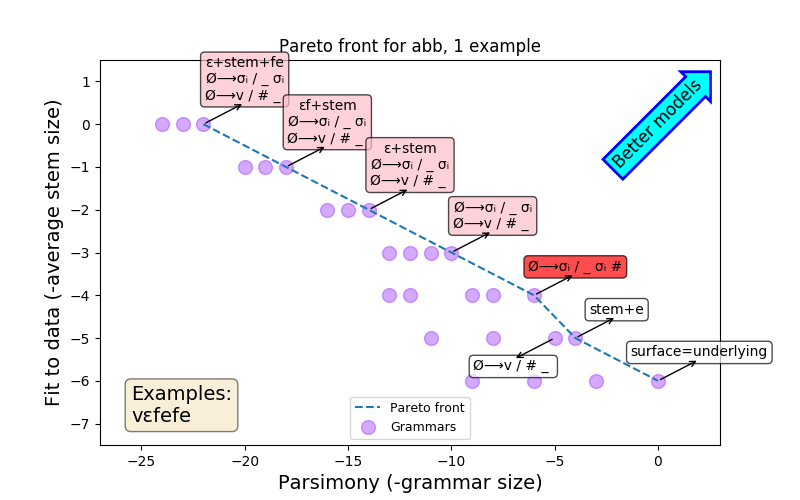
\includegraphics[width = 0.5\textwidth]{alternativeHypothesesFigures/abb1.png} 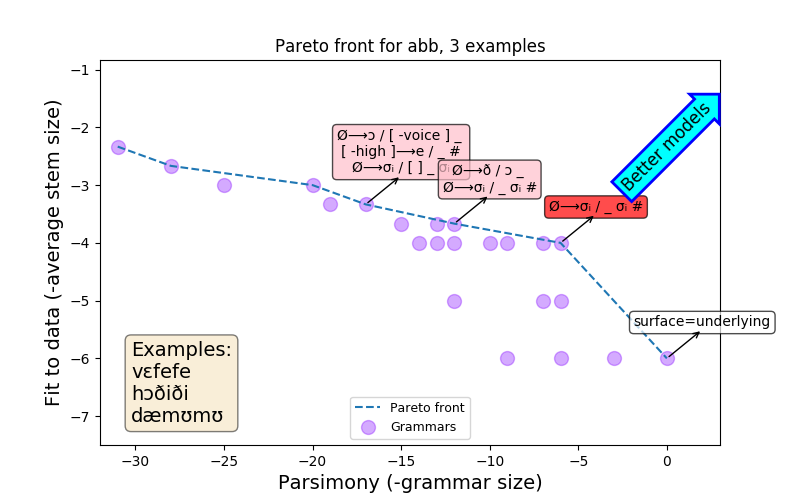
\includegraphics[width = 0.5\textwidth]{alternativeHypothesesFigures/abb3.png}
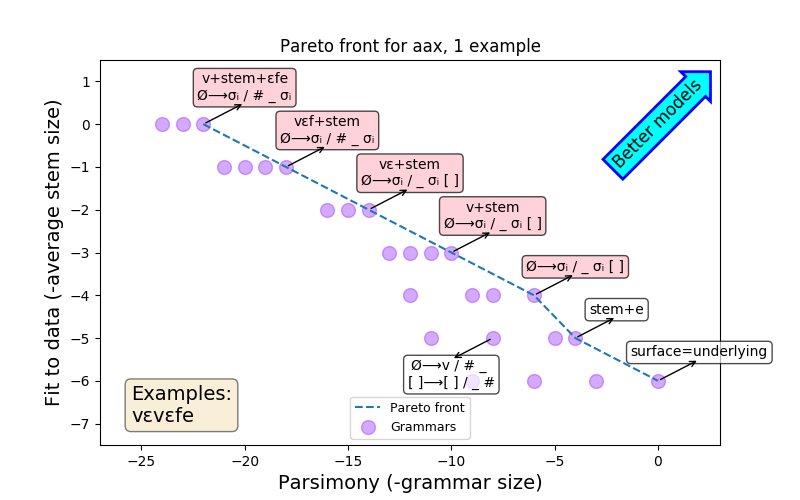
\includegraphics[width = 0.5\textwidth]{alternativeHypothesesFigures/aax1.png} 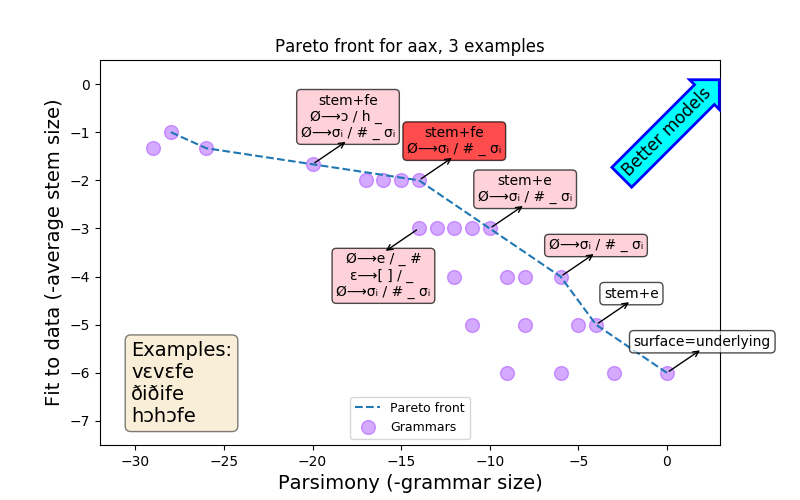
\includegraphics[width = 0.5\textwidth]{alternativeHypothesesFigures/aax3.png}
  
  \caption{Pareto fronts for ABB  (Marcus~1999; top two) \& AAX  (Gerken~2006; bottom two) learning problems fo either one example word (left column) or three example words  (right column). Rightward on x-axis corresponds to more parsimonious grammars and upward on y-axis corresponds to grammars that best fit the data, so the best grammars live in the upper right corners of the graphs. {\color{red}Red shade}: ground truth grammar. {\color{red!60}Pink shade}: shares structure with ground truth grammar. White shade: incorrect generalizations. As the number of examples increases, the Pareto fronts develop a sharp kink around the ground truth grammar, which indicates a stronger preference for the correct grammar. With one example the kinks can still exists but are less pronounced.}\label{quadrupleFrontier}
\end{figure}

\subsection{Beyond artificial grammars: Applying BPL to natural language}

A successful model of artificial grammar learning should also explain
at least some aspects of first language acquisition.  As a first step
in this direction, we take the same model that we applied to these AGL
learning problems and use it to solve phonology textbook exercises.
Each of these textbook exercises is an inductive reasoning problem
where the learner must explain surface pronunciations in terms of a
latent generative model (a grammar).

These natural language results are still preliminary and
ongoing. Figure~\ref{naturalLanguageExample} shows our model solving a
representative textbook problem.  We believe this extension to
natural language is an important next step for models of artificial
grammar learning, and helps deliver on the basic promises and
presuppositions of AGL research.



\begin{figure}[H]\centering
  \begin{minipage}{7cm}\centering
    \textbf{Textbook Tibetan counting problem:}
    \begin{tabular}{ll}\toprule
Number & Surface form
\\ \midrule
10 & \textipa{d\super Zu}\\
1 & \textipa{d\super Zig}\\
11 & \textipa{d\super Zugd\super Zig}\\
4 & \textipa{Si}\\
%14 & \textipa{d\super ZubSi}\\
40 & \textipa{Sibd\super Zu}\\
9 & \textipa{gu}\\
19 & \textipa{d\super Zurgu}\\
%90 & \textipa{gubd\super Zu}\\
5 & \textipa{Na}\\
%15 & \textipa{d\super ZuNa}\\
%50 & \textipa{Nabd\super Zu}\\
\bottomrule
\end{tabular}
  \end{minipage}%
  \hspace{0.25cm}
  \begin{minipage}{7cm}\centering
    \textbf{Our model's solution:}
    
    Induced phonological rule: \phonb{C}{$\varnothing $}{\#}{C} \\ %\texttt{C}$\to\varnothing /$\texttt{\#\_C} \\
    \hspace{0.5cm}\emph{(Reduce word initial consonant clusters)}

    Induced underlying representations:
\\\begin{tabular}{ll}\toprule
1 & \textipa{gd\super Zig}\\
4 & \textipa{bSi}\\
5 & \textipa{Na}\\
9 & \textipa{rgu}\\
10 & \textipa{bd\super Zu}
\bottomrule
\end{tabular}    
  \end{minipage}
  \caption{Example textbook phonology exercise (left, taken from~\cite{9780511808869}) and the solution our model discovers for it (right). To solve this problem the model must jointly infer unobserved underlying representations for each of the Tibetan numbers, along with a phonological rule that explains their surface pronunciations. The same code that calculated the Pareto fronts (Figure~\ref{quadrupleFrontier}) produces this analysis of the Tibetan count system.}\label{naturalLanguageExample}
  \end{figure}



\bibliographystyle{unsrt} \bibliography{main}


\end{document}
